%%%%%%%%%%%%%%%%%%%%%%%%%%%%%%%%%%%%%%%%%%%%%%%%%%%%%%%%%%%%%%%%%%%%%%
% predefined document class
%%%%%%%%%%%%%%%%%%%%%%%%%%%%%%%%%%%%%%%%%%%%%%%%%%%%%%%%%%%%%%%%%%%%%%
\documentclass[%
	%handout
]{phdpresentation}

%%%%%%%%%%%%%%%%%%%%%%%%%%%%%%%%%%%%%%%%%%%%%%%%%%%%%%%%%%%%%%%%%%%%%%
% inputs
%%%%%%%%%%%%%%%%%%%%%%%%%%%%%%%%%%%%%%%%%%%%%%%%%%%%%%%%%%%%%%%%%%%%%%
%%%%%%%%%%%%%%%%%%%%%%%%%%%%%%%%%%%%%%%%%%%%%%%%%%%%%%%%%%%%%%%%%%%%%%
\usepackage{datetime}
%%%%%%%%%%%%%%%%%%%%%%%%%%%%%%%%%%%%%%%%%%%%%%%%%%%%%%%%%%%%%%%%%%%%%%
\newcommand{\thesisTitle}{Mesoscale~Discrete~Element~Model for~Concrete and~Its~Combination~with~FEM}
\newcommand{\authorName}{Jan Stránský}
\newcommand{\authorDegree}{Ing.}
\newcommand{\thesisType}{doctoral thesis}
\newcommand{\university}{Czech~Technical University in~Prague}
\newcommand{\faculty}{Faculty of~Civil Engineering}
\newcommand{\department}{Department of Mechanics}
\newcommand{\address}{Thákurova 7, 166 29 Praha 6}
\newcommand{\PhDProgramme}{Civil Engineering}
\newcommand{\branchOfStudy}{Physical and Material Engineering}
\newcommand{\supervisor}{prof. Ing. Milan Jirásek, DrSc.}
\newcommand{\submissionPlace}{Prague}
\newcommand{\submissionYear}{2018}
\newcommand{\submissionMonth}{1}
\newcommand{\submissionDay}{31}
\newcommand{\submissionDate}{\ordinaldate{\submissionDay} \monthname[\submissionMonth] \submissionYear}
\newcommand{\periodOfDoctoralStudy}{1.2.2011 -- 31.1.2018}
\newcommand{\keywords}{Discrete Element Method, Finite Element Method, multimethod coupling, Python, concrete, mesoscale}
\newcommand{\keywordsCS}{Metoda diskrétních prvků, metoda konečných prvků, kombinování metod, Python, beton, mezoúroveň}
%%%%%%%%%%%%%%%%%%%%%%%%%%%%%%%%%%%%%%%%%%%%%%%%%%%%%%%%%%%%%%%%%%%%%%

\renewcommand{\abstract}{

The presented thesis deals with various aspects of the discrete element method (DEM) with application to modeling of concrete failure and combination of DEM with the finite element method (FEM).

% macromicro
Basic properties (e.g., isotropy) of random densely packed particle assemblies (as a~usual initial DEM packing configuration) are analyzed for various numbers of particles.
Elastic properties of such packings are investigated both analytically and numerically.
The analytical formulas are derived based on the microplane theory.
The numerical results are obtained by DEM and FEM simulations.
A very good agreement between analytical and numerical results is found for interaction ratios greater than $1{.}25$.
For lower values of the interaction ratio, the analytically derived full stiffness tensor corresponds to the numerical results very well, however, the values of Young's modulus and Poisson's ratio estimated based on the assumption of uniform distribution of link directions exhibit a certain discrepancy from the numerical results.

% discrete stress
The discrete nature is an essential feature of DEM.
However, in some cases it is desirable to transform such discrete information (contact forces for instance) into its continuum counterpart (e.g., stress tensor).
The evaluation of the stress tensor and couple stress tensor from discrete forces based on the principle of virtual work is reviewed.
New formulas for the couple stress tensor, yielding a unique value of the couple stress tensor independent on the choice of the coordinate reference point, are presented and discussed.

% concurrent coupling
Both DEM and FEM have their fields of application, however, in certain cases they can be combined and used together.
In the concurrent coupling approach, both DEM and FEM simulations are run at the same time.
Coupling of FEM code \OOFEM\ and DEM code \YADE\ is described.
Several classes of coupling approaches (namely surface, direct volume, multiscale and contact) are addressed and illustrated on simple examples.

% sequential coupling
A DEM to FEM sequential coupling (in which case the DEM simulation is run first and the resulting state is converted into an initial state of the FEM simulation) of damaged concrete material is presented for the case of uniaxial compression.
The method is proven to be able to capture the transition from DEM to FEM relatively well for several different loading scenarios -- mapping at different stages (elastic range, peak load, softening regime, with or without unloading etc.).
The most divergent results are obtained for the stages of loading where the DEM and FEM material models themselves differ the most.

% mcpm
In practical civil engineering, concrete is usually idealized as a homogeneous isotropic material.
However, certain applications require description of concrete on a lower scale and heterogeneity has to be taken into account.
The development and results of a new mesoscale discrete element model for concrete is described.
The model takes into account the heterogeneous mesoscale structure of concrete (i.e., aggregates and interfacial transition zone between aggregates and matrix).
The validation against experimental data from literature shows the ability of the model to realistically capture trends of various material properties (elastic modulus, tensile and compressive strength, fracture energy) with respect to the actual mesoscale structure of the material.
}



\newcommand{\abstractCS}{

Dizertační práce se zabývá různými aspekty metody diskrétních prvků (DEM) a její aplikací pro modelování porušování betonu
a také kombinací DEM s metodou konečných prvků (FEM).

% macromicro
Základní vlastnosti náhodných hustých částicových shluků (jelikož tyto jsou obvyklé počáteční nastavení DEM simulací) jsou analyzovány pro různý počet částic.
Pružné vlastnosti takovýchto shluků jsou zkoumány analyticky i numericky.
Numerické výrazy jsou odvozeny na základě mikroploškové teorie.
Numerické výsledky jsou získány pomocí DEM a FEM simulací.
Velmi dobré shody mezi analytickými a numerickými výcledky je dosaženo pro interakční poměr větší než 1{.}25.
Analyticky odvozený plný tenzor pružné tuhosti se velmi dobře shoduje s numerickými výsledky i pro nižší hodnoty interakčního poměru, avšak hodnoty Youngova modulu pružnosti a Poissonova součinitele odvozené za předpokladu rovnoměrného rozdělení směrů vazeb vykazuje jistou odchylku od numerických výsledků.

% discrete stress
Nespojitost je základní vlastností DEM.
V některých situacích je však žádoucí převěst nespojité veličiny (např. síly) na odpovídajíci spojitou veličinu (např. tenzor napětí).
Je představeno vyhodnocení tenzoru napětí a couple stress tenzoru z nespojitých sil.
Metoda je založena na principu virtuálních prací.
Jsou představeny nové výrazy pro couple stress tenzor, jejíchž výsledek je jedinečný a nezávislý na volbě pořátku souřadnicového systému.

% concurrent coupling
DEM i FEM mají své oblasti použití, někdy mohou ale spolu mohou být vhodně zkombinovány.
V souběžných kombinačních přístupech běží DEM i FEM simulace současně.
Je představena kombinace FEM programu \OOFEM\ a DEM programu \YADE.
Je popsáno několik různých přístupů (jmenovitě povrchové, objemové, víceúrovňové a kontektní), každý z nich ilustrovaný na jednoduchém případě.

% sequential coupling
Sériová DEM--FEM kombinace (kdy DEM simulace probíhá první a její výsledek je převeden jako počáteční stav FEM simulace) poškozujícího se betonového materiálu je představena na příkladu jednoosého tlaku.
Metoda prokázala schopnost poměrně dobře vystihnout přechod z DEM do FEM pro různé módy zatížení -- mapování v různých stádiích (průžná oblast, vrchol pevnosti, změkkčení atd.).
Výsledky se nejvíse liší v těch oblastech zatížení, kde se samotné DEM a FEM materiálové modely liší nejvíce.

% mcpm
Ve stavební praxi je beton obvykle idealizován jako homogenní izotropní materiál.
Některé aplikace však vyžadují popis betonu na nižší úrovni a musí se uvažovat nestejnorodosti.
Je představen vývoj a výsledky nového mezoúrovňového modelu pro beton.
Model uvažuje nestejnorodou mezoúroveň betonu (t.j. zrna kameniva a zónu rozhraní mezi kamenivem a matricí).
Validace vzhledem k experimentálním výsledkům přebraným z literatury prokázala schopnost modelu realisticky vystihnout trendy různých materiálových vlastností (modulu pružnosti, tahové a tlakové pevnosti, lomové energie) vzhledem k mezo\-úrovňové struktuře materiálu.
}

\usepackage[multidit]{grffile} % dots in input names
\usepackage{xifthen}
\usepackage{mathtools}
\usepackage{scalerel}
\usepackage{array}

\graphicspath{{../figs/}{../figs/ctu/}{plots/}}

\newcommand{\quotes}[1]{``#1''}

\newcommand{\code}[1]{\texttt{#1}}
\newcommand{\textfile}[1]{\texttt{#1}}

\unitlength=1mm

\newcolumntype{C}[1]{>{\centering\arraybackslash}m{#1}}
\renewcommand{\arraystretch}{1.2}

\newcommand{\inputplot}[1]{\input{plots/plots/#1}}

\newcommand{\dd}[1]{\text{d}#1}
\newcommand{\idd}[1]{\,\text{d}#1}
\newcommand{\bb}[1]{{\bf #1}}
\newcommand{\oo}[1]{\overline{#1}}
\newcommand{\uu}[1]{\underline{#1}}
\newcommand{\T}[1][]{^{#1\mathsf{T}}}
\newcommand{\sym}[1]{#1^{\mathsf{S}}}
\newcommand{\antisym}[1]{#1^{\mathsf{A}}}
\newcommand{\vol}[1]{#1^{\mathsf{V}}}
\newcommand{\dev}[1]{#1^{\mathsf{D}}}
\newcommand{\abs}[1]{\left|#1\right|}

\newcommand{\arrow}{}
\let\arrow\vector

\renewcommand{\vector}[1]{\bbb{#1}}
\newcommand{\mat}[1]{\bbb{#1}}

% https://tex.stackexchange.com/questions/194798/change-vertical-space-in-overset
\makeatletter
\newcommand{\oset}[3][0ex]{%
	\mathrel{\mathop{#3}\limits^{
		\vbox to#1{\kern-2\ex@
		\hbox{$\scriptstyle#2$}\vss}}}}
\makeatother
\newcommand{\cdotMiddle}{\oset[-.1em]{m}{\boldsymbol{\cdot}}}

% https://tex.stackexchange.com/questions/199333/turn-mathbb-characters-bold-in-math-mode
\newcommand{\fakebold}[2][.3pt]{
	\ThisStyle{\ooalign{$\SavedStyle#2$\cr%
	\kern-#1$\SavedStyle#2$\cr%
	\kern.0pt$\SavedStyle#2$\cr%
	\kern#1$\SavedStyle#2$}}%
}
\newcommand{\bbb}[1]{%
	\expandafter\ifstrequal{#1}{varepsilon}{\fakebold[.9pt]{#1}}{%
		\IfSubStr{ABCDEFGHIJKLMNOPQRSTUVWXYZabcdefghijklmnopqrstuvwxyz}{#1}
			{{\bf #1}}
			{\boldsymbol{#1}}
	}
}

\newcommand{\tensor}[2]{%
	\ifthenelse{\equal{#1}{0}}{ #2 }{}%
	\ifthenelse{\equal{#1}{1}}{ \vector{#2} }{}%
	\ifthenelse{\equal{#1}{2}}{ \mat{#2} }{}%
	\ifthenelse{\equal{#1}{3}}{ \bbb{\mathcal{#2}} }{}%
	\ifthenelse{\equal{#1}{4}}{ \fakebold[.35pt]{\mathbb{#2}} }{}%
}

\newcommand{\interactionRatio}{\iota_r}
\newcommand{\strain}{\varepsilon}
\newcommand{\stress}{\sigma}
\newcommand{\matB}{\mat{B}}
\newcommand{\matT}{\mat{T}}
\newcommand{\position}{x}
\newcommand{\positionVector}{\tensor1{\position}}
\newcommand{\particlePosition}{\vector{p}}
\newcommand{\normal}{n}
\newcommand{\normalVector}{\tensor1{\normal}}
\newcommand{\normalTensor}[1]{\tensor{#1}{N}}
\newcommand{\shearTensor}[1]{\tensor{#1}{T}}
\newcommand{\stiffness}{D}
\newcommand{\compliance}{C}
\newcommand{\elastic}{_e}
\newcommand{\inv}{^{-1}}
\newcommand{\stiffnessTensor}{\tensor4{\stiffness}}
\newcommand{\stiffnessTensorElastic}{\stiffnessTensor\elastic}
\newcommand{\complianceTensor}{\tensor4{\compliance}}
\newcommand{\complianceTensorElastic}{\complianceTensor\elastic}
\newcommand{\stressTensor}{\tensor2{\stress}}
%\newcommand{\strainTensor}{\tensor2{\strain}}
\newcommand{\strainTensor}{\fakebold[.1pt]{\tensor2{\strain}}}
\newcommand{\elementStiffnessMatrix}{\mat{K}}
\newcommand{\materialStiffnessMatrix}{\mat{\stiffness}}
\newcommand{\stiffnessMatrix}{\materialStiffnessMatrix}
\newcommand{\stiffnessMatrixElastic}{\stiffnessMatrix\elastic}
\newcommand{\complianceMatrix}{\mat{\compliance}}
\newcommand{\complianceMatrixElastic}{\complianceMatrix\elastic}
%\newcommand{\strainVector}{\vector{\strain}}
\newcommand{\strainVector}{\fakebold[.1pt]{\vector{\strain}}}
\newcommand{\displacement}{u}
\newcommand{\displacementVector}{\vector{\displacement}}
\newcommand{\force}{f}
\newcommand{\forceVector}{\vector{\force}}
\newcommand{\couple}{c}
\newcommand{\coupleVector}{\vector{\couple}}
\newcommand{\radius}{r}
\newcommand{\normalComponent}{N}
\newcommand{\shearComponent}{T}
\newcommand{\rotation}{\phi}
\newcommand{\Rotation}{\Phi}
%\newcommand{\rotationVector}{\vector{\rotation}}
\newcommand{\rotationVector}{\fakebold[.2pt]{\vector{\rotation}}}
\newcommand{\rotationTensor}{\vector{\Rotation}}

\newcommand{\volume}{V}
\newcommand{\dVolume}{\idd{\volume}}
\newcommand{\surface}{S}
\newcommand{\dSurface}{\idd{\surface}}
\newcommand{\solidAngle}{\Omega}
\newcommand{\dSolidAngle}{\idd{\Omega}}
\newcommand{\azimuthAngle}{\theta}
\newcommand{\dAzimuthAngle}{\idd{\azimuthAngle}}
\newcommand{\zenithAngle}{\varphi}
\newcommand{\dZenithAngle}{\idd{\zenithAngle}}
\newcommand{\primitiveFunctionWithLimits}[3]{\left[#1\right]_{#2}^{#3}}
\newcommand{\bnabla}{\boldsymbol{\nabla}}
\newcommand{\coordinateVector}{\tensor1{x}}

\newcommand{\identity}{I}
\newcommand{\identityTensor}[1]{%
	\ifthenelse{\equal{#1}{2}}{ \tensor2{1} }{}%
	\ifthenelse{\equal{#1}{4}}{ \tensor4{\identity} }{}%
}
\newcommand{\projection}{I}
\newcommand{\projectionTensor}[1]{%
	\ifthenelse{\equal{#1}{4}}{ \tensor4{\projection} }{}%
}
\newcommand{\LeviCivita}{\tensor3{E}}
\newcommand{\leviCivita}[1]{\varepsilon_{#1}}
\newcommand{\trace}[1]{\text{tr}\!\left(#1\right)}
\newcommand{\kdelta}[1]{\delta_{#1}}

\newcommand{\complexity}[1]{O(#1)}


\newcommand{\linkLength}{\branch}
\newcommand{\linkCrossSectionArea}{A}
\newcommand{\linkCrossSectionAreaFactor}{\alpha}
\newcommand{\linkMaterialStiffnessNormal}{\skew{5}{\bar}{\youngModulus}}
\newcommand{\linkMaterialStiffnessShear}{\skew{5}{\bar}{\shearModulus}}
\newcommand{\linkStiffness}{\skew{5}{\bar}{k}}
\newcommand{\linkStiffnessNormal}{\linkStiffness_\normalComponent}
\newcommand{\linkStiffnessShear}{\linkStiffness_\shearComponent}
\newcommand{\linkStrainVector}{\vector{\strain}}
\newcommand{\linkStrainNormal}{\strain_\normalComponent}
\newcommand{\linkStrainNormalVector}{\vector{\strain}_\normalComponent}
\newcommand{\linkStrainShear}[1][]{\strain_{\shearComponent#1}}
\newcommand{\linkStrainShearVector}{\vector{\strain}_\shearComponent}
\newcommand{\linkStrainShearVectorPlastic}{\linkStrainShearVector^p}
\newcommand{\linkStrainShearVectorPlasticRate}{\dot{\vector{\strain}}_\shearComponent^p}
\newcommand{\linkNodalDsplVector}{\vector{d}}
\newcommand{\linkStrainDisplacementMatrix}{\mat{B}}
\newcommand{\linkMaterialStiffnessMatrix}{\mat{D}}
\newcommand{\linkStressVector}{\vector{\stress}}
\newcommand{\linkStressShearVector}{\vector{\stress}_\shearComponent}
\newcommand{\linkStressNormal}{\stress_\normalComponent}
\newcommand{\linkStressShear}[1][]{\stress_{\shearComponent#1}}
\newcommand{\linkNodalForceVector}{\vector{f}}
\newcommand{\linkStiffnessMatrix}{\mat{K}}
\newcommand{\nodalDsplVector}{\linkNodalDsplVector}
\newcommand{\lcs}{l}
\newcommand{\gcs}{g}
\newcommand{\linkGlobToLoc}{\mat{R}}
\newcommand{\linkGlobToLocE}{\vector{e}}
\newcommand{\linkTrsfMat}{\mat{T}}
\newcommand{\linkDisplacementNormal}{\displacement_\normalComponent}
\newcommand{\linkDisplacementNormalVector}{\displacementVector_\normalComponent}
\newcommand{\linkDisplacementShear}[1][]{\displacement_{\shearComponent#1}}
\newcommand{\linkDisplacementShearVector}{\displacementVector_\shearComponent}
\newcommand{\contact}{c}
\newcommand{\contactPoint}{\tensor1{\contact}}

\newcommand{\particle}{P}
\newcommand{\particleA}{J}
\newcommand{\particleB}{K}

\newcommand{\cubeDimension}{C}
\newcommand{\cubeVolume}{V}
\newcommand{\youngModulus}{E}
\newcommand{\poissonRatio}{\nu}
\newcommand{\numberOfParticles}{N}
\newcommand{\numberOfContacts}{N_\contact}

\newcommand{\packingFraction}{PF}

\newcommand{\cross}{\times}
\newcommand{\norm}[1]{|\!|#1|\!|}

\newcommand{\arrowWithSpaces}{\quad\rightarrow\quad}
\newcommand{\rr}{\arrowWithSpaces}
\newcommand{\avg}{\mathsf{avg}}
\newcommand{\shearModulus}{G}

\newcommand{\macroscopicDeformation}{E}
\newcommand{\macroscopicDeformationVector}{\vector{\macroscopicDeformation}}

\newcommand{\deformationGradient}{\tensor2{F}}
\newcommand{\coupleStress}{\mu}
\newcommand{\coupleStressTensor}{\tensor2{\coupleStress}}
\newcommand{\surfForce}{t}
\newcommand{\surfForceVector}{\tensor1{t}}
\newcommand{\bodyForce}{f}
\newcommand{\bodyForceVector}{\tensor1{\bodyForce}}
\newcommand{\bodyCouple}{c}
\newcommand{\bodyCoupleVector}{\tensor1{\bodyCouple}}
\newcommand{\surfCouple}{m}
\newcommand{\surfCoupleVector}{\tensor1{\surfCouple}}

\newcommand{\curvature}{\kappa}
\newcommand{\curvatureTensor}{\tensor2{\curvature}}
\newcommand{\Displacement}{U}
\newcommand{\displacementGradient}{\tensor2{\Displacement}}
\newcommand{\virtual}{\delta}

\newcommand{\work}{W}
\newcommand{\virtualWork}{\virtual\work}

\newcommand{\volumeAverage}[1]{\overline{#1}}

\newcommand{\external}[1]{#1^e}
\newcommand{\internal}[1]{#1^c}
\newcommand{\externalForceVector}{\external{\tensor1{f}}}
\newcommand{\externalCoupleVector}{\external{\tensor1{c}}}
\newcommand{\internalForceVector}{\internal{\tensor1{f}}}
\newcommand{\internalCoupleVector}{\internal{\tensor1{c}}}

\newcommand{\firstMomentOfVolumeVector}{\tensor1{s}}

\newcommand{\subsubsubsection}[1]{\paragraph{#1}}
\newcommand{\externalp}{e}
\newcommand{\branch}{L}
\newcommand{\branchVector}{\tensor1{l}}

\newcommand{\centroidVector}{\positionVector^0}

\newcommand{\matTPeri}{\mat{P}}
\newcommand{\periodicShift}{k}

\newcommand{\mass}{m}
\newcommand{\acceleration}{\ddot{\displacement}}
\newcommand{\accelerationVector}{\ddot{\displacementVector}}
\newcommand{\angularAcceleration}{\ddot{\rotation}}
\newcommand{\angularAccelerationVector}{\ddot{\rotationVector}}
\newcommand{\inertiaTensor}{\tensor2{I}}

\newcommand{\damage}{\omega}
\newcommand{\Damage}{\Omega}
\newcommand{\damageTensor}{\tensor2{\Damage}}
\newcommand{\stressTensorEffective}{\overline{\stressTensor}}
\newcommand{\plastic}{_p}
\newcommand{\strainTensorPlastic}{\strainTensor\plastic}
\newcommand{\strainTensorPlasticRate}{\dot{\strainTensor}\plastic}
\newcommand{\strainTensorElastic}{\strainTensor\elastic}
\newcommand{\kappaP}{\kappa_P}
\newcommand{\kappaD}{\kappa_D}
\newcommand{\damageA}{\hat{\damage}}
\newcommand{\damageTensorI}{\Damage}

\newcommand{\Time}{t}
\newcommand{\damageEvolutionFunction}{g}
\newcommand{\strainO}{\strain_0}
\newcommand{\strainF}{\strain_f}
\newcommand{\cohesion}{c}
\newcommand{\cohesionInitial}{\cohesion_0}
\newcommand{\frictionAngle}{\varphi}
\newcommand{\br}[1]{\left(#1\right)}

\newcommand{\velocity}{v}
\newcommand{\velocityVector}{\vector{\velocity}}
\newcommand{\angularVelocity}{\omega}
\newcommand{\angularVelocityVector}{\vector{\angularVelocity}}

\newcommand{\halfBranch}{d}

\newcommand{\OOFEM}{OOFEM}
\newcommand{\YADE}{YADE}
\newcommand{\github}{GitHub}
 % user defined commands

%%%%%%%%%%%%%%%%%%%%%%%%%%%%%%%%%%%%%%%%%%%%%%%%%%%%%%%%%%%%%%%%%%%%%%
% field setting in PDF document
%%%%%%%%%%%%%%%%%%%%%%%%%%%%%%%%%%%%%%%%%%%%%%%%%%%%%%%%%%%%%%%%%%%%%%
\hypersetup{
	pdftitle={\thesisTitle},%
	pdfauthor={\authorName},%
	pdfcreator={\authorName},%
	pdfproducer={\authorName},%
	pdfsubject={Doctoral thesis defense presentation},%
	pdfkeywords={\keywords}%
}

\title{\thesisTitle}
\author{\authorName}
\institute{\department\par\faculty\par\university}
\date{\defenseDate}


%%%%%%%%%%%%%%%%%%%%%%%%%%%%%%%%%%%%%%%%%%%%%%%%%%%%%%%%%%%%%%%%%%%%%%
\begin{document}

% titlepage
\begin{frame}
	\clearpage
	\thispagestyle{empty}
	\vspace*{5mm}
	\titlepage
\end{frame}

% outline
\outlineframe

%%%%%%%%%%%%%%%%%%%%%%%%%%%%%%%%%%%%%%%%%%%%%%%%%%%%%%%%%%%%%%%%%%%%%%
% D E M
%%%%%%%%%%%%%%%%%%%%%%%%%%%%%%%%%%%%%%%%%%%%%%%%%%%%%%%%%%%%%%%%%%%%%%
\section{Discrete element method}
\begin{frame}
	\frametitle{\secname\ (DEM)}
	\begin{twocolumns}
		\begin{onecolumn}
			\begin{myitemize}
				\item<1-> set of rigid particles
				\item<1-> various particle shapes
				\item<3-> motion, contact detection
				\item<3-> Newton's laws of motion
				\item<10-> contact laws
			\end{myitemize}
		\end{onecolumn}
		\begin{onecolumn}
			\only<1| handout:0>{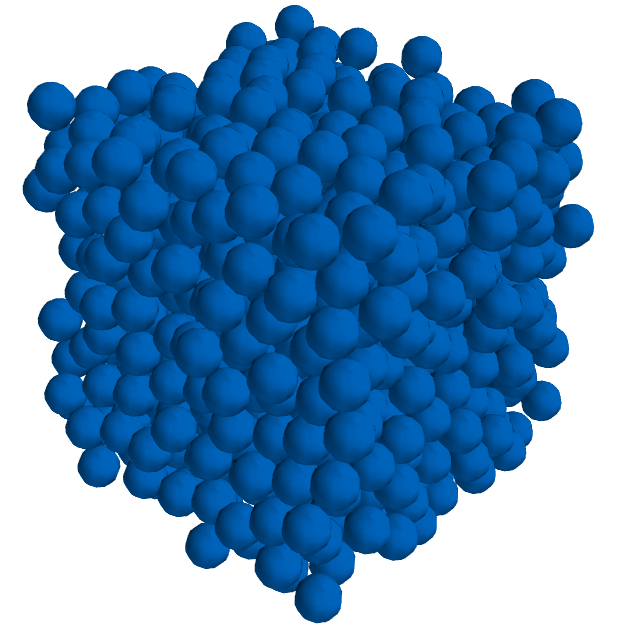
\includegraphics[width=\textwidth]{figs/packing}}
			\only<2| handout:0>{\includegraphics[width=\textwidth]{figs/raphaelpy/particle_shapes}}
			\only<3| handout:0>{\includegraphics[width=\textwidth]{figs/raphaelpy/dem_illustration_0}}
			\only<4| handout:0>{\includegraphics[width=\textwidth]{figs/raphaelpy/dem_illustration_1}}
			\only<5| handout:0>{\includegraphics[width=\textwidth]{figs/raphaelpy/dem_illustration_2}}
			\only<6| handout:0>{\includegraphics[width=\textwidth]{figs/raphaelpy/dem_illustration_3}}
			\only<7| handout:0>{\includegraphics[width=\textwidth]{figs/raphaelpy/dem_illustration_4}}
			\only<8| handout:0>{\includegraphics[width=\textwidth]{figs/raphaelpy/dem_illustration_5}}
			\only<9| handout:0>{\includegraphics[width=\textwidth]{figs/raphaelpy/dem_illustration_6}}
			\only<10| handout:1>{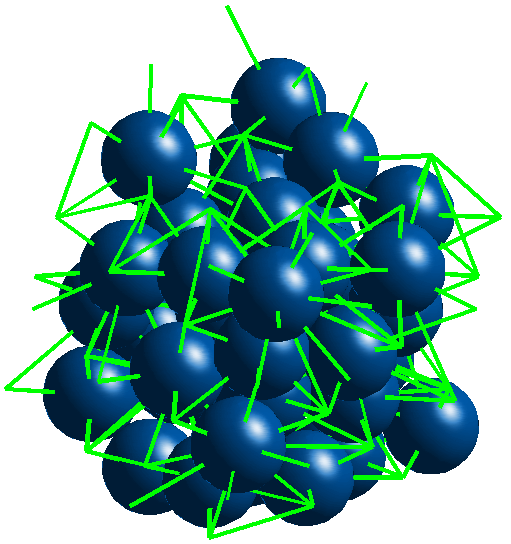
\includegraphics[width=\textwidth]{figs/packing_with_links}}
		\end{onecolumn}
	\end{twocolumns}
\end{frame}

\subsection{Particle model for concrete}
\begin{frame}
	\frametitle{\secname}
	\framesubtitle{\subsecname}
	\begin{twocolumns}
		\begin{onecolumn}
			\begin{myitemize}
				\item<1-> by Šmilauer \& Jirásek
				\item<2-> uniform spheres
				\item<2-> artificial discretization
				\item<2-> random close packing
				\item<2-> cohesive links
				\item<3-> interaction ratio
				\item<7-> normal and shear stress
				\item<8-> damage and plasticity
				\item<9-> uniaxial tests illustration
			\end{myitemize}
		\end{onecolumn}
		\begin{onecolumn}
			\only<2| handout:0>{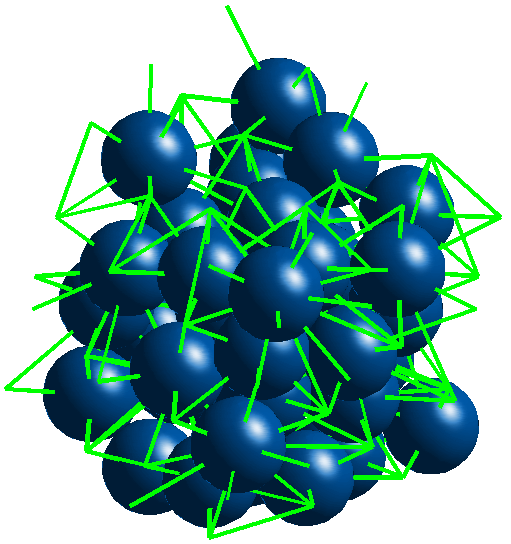
\includegraphics[width=\textwidth]{figs/packing_with_links}}
			\only<3| handout:0>{\includegraphics[width=\textwidth]{figs/raphaelpy/interaction_ratio_0}}
			\only<4| handout:0>{\includegraphics[width=\textwidth]{figs/raphaelpy/interaction_ratio_1}}
			\only<5| handout:0>{\includegraphics[width=\textwidth]{figs/raphaelpy/interaction_ratio_2}}
			\only<6| handout:0>{\includegraphics[width=\textwidth]{figs/raphaelpy/interaction_ratio_3}}
			\only<7| handout:0>{\includegraphics[width=\textwidth]{figs/raphaelpy/normal_shear_dir}}
			\only<8| handout:1>{
				\inputplot{cpm_law_tester_normal_simple_tension}
				\inputplot{cpm_shear_plasticity_func}
			}
			\only<9| handout:0>{\inputplot{cpm_uniax_tension}}
			\only<10| handout:0>{\inputplot{cpm_uniax_compression}}
		\end{onecolumn}
	\end{twocolumns}
\end{frame}


%%%%%%%%%%%%%%%%%%%%%%%%%%%%%%%%%%%%%%%%%%%%%%%%%%%%%%%%%%%%%%%%%%%%%%
% E L A S T I C
%%%%%%%%%%%%%%%%%%%%%%%%%%%%%%%%%%%%%%%%%%%%%%%%%%%%%%%%%%%%%%%%%%%%%%
\section{Macroscopic elastic properties of DEM models}
\begin{frame}
	\frametitle{\secname}
	\begin{twocolumns}
		\begin{onecolumn}
			micro parameters: $\linkMaterialStiffnessNormal$, $\linkMaterialStiffnessShear$ \par
			macro parameters: $\youngModulus$, $\poissonRatio$ \par
			\uncover<2->{
				\begin{block}{Numerical solution}
					\begin{myitemize}
						\item dynamic DEM, static FEM
						\item periodic BCs
					\end{myitemize}
				\end{block}
			}
			\uncover<3->{
				\begin{block}{Analytical solution}
					\begin{myitemize}
						\item<3-> affine displacement
						\item<5-> stiffness tensor
						\item<6-> uniform distribution of link directions
					\end{myitemize}
				\end{block}
			}
		\end{onecolumn}
		\begin{onecolumn}
			\only<1| handout:0>{
				\includegraphics[width=4cm]{figs/raphaelpy/normal_shear_dir}
				\begin{picture}(0,0)
					\setlength{\unitlength}{1cm}
					\put(-2.5,1.7){\makebox(0,0){$\linkMaterialStiffnessNormal$}}
					\put(-1.8,2.0){\makebox(0,0){$\linkMaterialStiffnessShear$}}
				\end{picture}
				\par
				\vspace{3mm}
				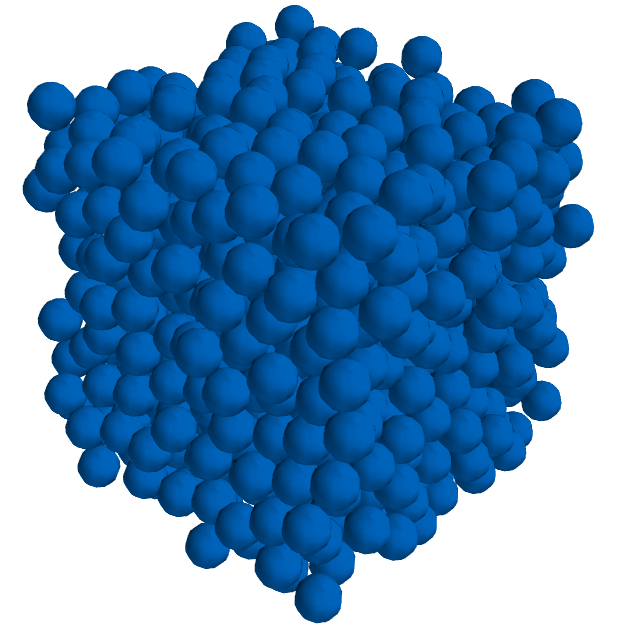
\includegraphics[width=4cm]{figs/packing}
				\begin{picture}(0,0)
					\setlength{\unitlength}{1cm}
					\put(-.5,.7){\makebox(0,0){$\youngModulus, \poissonRatio$}}
				\end{picture}
			}
			\only<2| handout:0>{
				\includegraphics[width=4cm]{../figs/raphaelpy/peri_packing_2d_illustration_0}
				\setlength{\unitlength}{4cm}
				\put(-0.615384615385,0.384615384615){\makebox(0,-.01)[lt]{$\particleA$}}
				\put(-0.230769230769,0.769230769231){\makebox(0,0)[l]{$\particleA'$}}
				\put(-0.394230769231,0.605769230769){\makebox(0,-.02)[lt]{$\particleB$}}
				\put(-0.778846153846,0.221153846154){\makebox(0,-.02)[t]{$\particleB'$}}
			}
			\only<3| handout:0>{\includegraphics[width=\textwidth]{figs/raphaelpy/affine_dspl_0}}
			\only<4| handout:0>{\includegraphics[width=\textwidth]{figs/raphaelpy/affine_dspl_1}}
			\only<5-| handout:1>{
				$$
					\stiffnessTensorElastic =
					\frac{1}{\volume} \sum_\contact \branch^\contact\linkCrossSectionArea^\contact\br{\linkMaterialStiffnessNormal\normalTensor4^\contact+\linkMaterialStiffnessShear\shearTensor4^\contact}
				$$
				\uncover<6-| handout:1>{
					\vspace{1cm}
					$$
						\youngModulus =
						\frac{\sum\branch^\contact\linkCrossSectionArea^\contact}{3\volume}
						\cdot
						\frac{\linkMaterialStiffnessNormal\br{2\linkMaterialStiffnessNormal+3\linkMaterialStiffnessShear}}{4\linkMaterialStiffnessNormal+\linkMaterialStiffnessShear}
					$$
					$$
						\poissonRatio = \frac{\linkMaterialStiffnessNormal-\linkMaterialStiffnessShear}{4\linkMaterialStiffnessNormal+\linkMaterialStiffnessShear}
					$$
				}
			}
		\end{onecolumn}
	\end{twocolumns}
\end{frame}

\subsection{Results}
\begin{frame}
	\frametitle{\secname}
	\framesubtitle{\subsecname}
	\only<1>{
		interaction ratio = 1.50 \par
		\inputplot{preprocessed_macromicro_E_I1.50}
		\inputplot{preprocessed_macromicro_nu_I1.50}
	}
	\only<2| handout:0>{
		interaction ratio = 1.05 \par
		\inputplot{preprocessed_macromicro_E_I1.05}
		\inputplot{preprocessed_macromicro_nu_I1.05}
	}
\end{frame}


%%%%%%%%%%%%%%%%%%%%%%%%%%%%%%%%%%%%%%%%%%%%%%%%%%%%%%%%%%%%%%%%%%%%%%
% D E M  -  F E M  C O U P L I N G
%%%%%%%%%%%%%%%%%%%%%%%%%%%%%%%%%%%%%%%%%%%%%%%%%%%%%%%%%%%%%%%%%%%%%%
\section{DEM -- FEM coupling}
\begin{frame}
	\frametitle{\secname}
	\framesubtitle{Motivation}
	\begin{twocolumns}
		\begin{onecolumn}
			\begin{block}{DEM}
				discrete domains\par
				\vspace{2mm}
				\centering
				\includegraphics[width=\textwidth]{figs/raphaelpy/ballast}
			\end{block}
		\end{onecolumn}
		\begin{onecolumn}
			\begin{block}{FEM}
				continuous domains\par
				\vspace{2mm}
				\centering
				\includegraphics[width=\textwidth]{figs/raphaelpy/sleeper}
			\end{block}
		\end{onecolumn}
	\end{twocolumns}
	\par
	\visible<2->{
		\begin{block}{Combination}
			\begin{myitemize}
				\item monolithic application -- redoing what already exists
				\item {\color{ctuRed}combination of existing codes}
			\end{myitemize}
			\vspace{1mm}
			\centering
			\includegraphics[width=.5\textwidth]{figs/raphaelpy/sleeper_ballast}
		\end{block}
	}
\end{frame}

\newcommand{\boxwh}[3]{\vbox to #2{\vfil\hbox to #1{#3}\vfil}}
\begin{frame}
	\frametitle{\secname}
	\framesubtitle{Motivation}
	\begin{twocolumns}
		\begin{onecolumn}
			\begin{block}{YADE}
				\boxwh{\textwidth}{2cm}{\hfill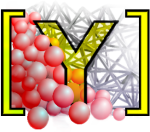
\includegraphics[height=2cm]{figs/yade-logo}\hfill}
				\begin{myitemize}
					\item<2-> DEM analysis
					\item<3-> free
					\item<4-> open source
					\item<5-> C++ core
					\item<6-> Python user interface
				\end{myitemize}
			\end{block}
		\end{onecolumn}
		\begin{onecolumn}
			\begin{block}{OOFEM}
				\boxwh{\textwidth}{2cm}{\centering
\includegraphics[width=\textwidth]{figs/oofem-logo}}
				\begin{myitemize}
					\item<2-> FEM analysis
					\item<3-> free
					\item<4-> open source
					\item<5-> C++ core
					\item<6-> Python user interface
				\end{myitemize}
			\end{block}
		\end{onecolumn}
	\end{twocolumns}
	\only<7| handout:0>{
		\vspace{-3cm}
		\centering
		\includegraphics[width=5cm]{figs/raphaelpy/hand_shaking}
	}
\end{frame}


\subsection{Surface coupling}
\begin{frame}
	\frametitle{\secname}
	\framesubtitle{\subsecname}
	\centering
	\includegraphics[width=6cm]{../figs/raphaelpy/coupling_illustration_surface}
	\begin{picture}(0,0)
		\setlength{\unitlength}{6cm}
		\put(-0.230769230769,0.0307692307692){\makebox(0,0){\small FEM}}
		\put(-0.830769230769,0.0307692307692){\makebox(0,0){\small DEM}}
		\put(-0.523076923077,0.446153846154){\makebox(0,0){\footnotesize load}}
		\put(-0.523076923077,0.2){\makebox(0,0){\footnotesize displacement}}
	\end{picture}
\end{frame}

\begin{frame}
	\frametitle{\secname}
	\framesubtitle{\subsecname}
	\centering
	\href{run:figs/surf1.gif}{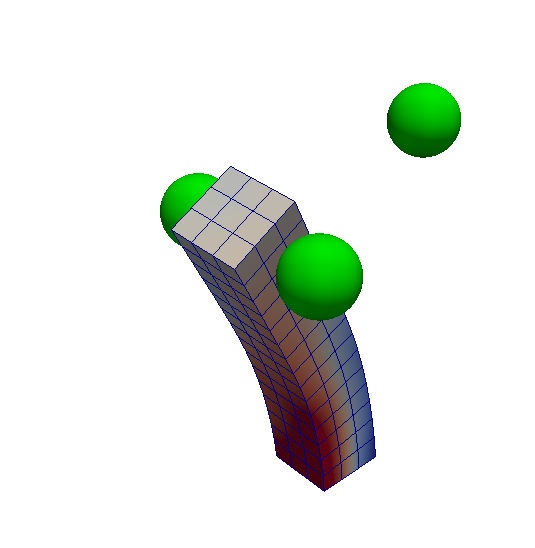
\includegraphics[height=7cm]{coupling/surf1/spheres/surf1-0030}}
\end{frame}

 
\subsection{Volume coupling}
\begin{frame}
	\frametitle{\secname}
	\framesubtitle{\subsecname}
	\centering
	\includegraphics[width=8cm]{../figs/raphaelpy/coupling_illustration_volume}
\end{frame}

\begin{frame}
	\frametitle{\secname}
	\framesubtitle{\subsecname}
	\centering
	\href{run:figs/vol1.gif}{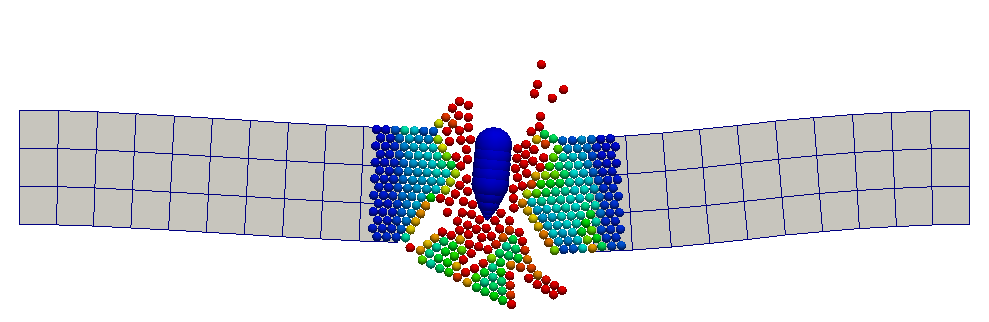
\includegraphics[width=10cm,trim={0 .0cm 0 2cm},clip]{coupling/vol1/vol1-0087}}
\end{frame}


\subsection{FE$\times$DE (multiscale) coupling}
\begin{frame}
	\frametitle{\secname}
	\framesubtitle{\subsecname}
	\centering
	\includegraphics[width=10cm]{../figs/raphaelpy/coupling_illustration_multiscale}
	\begin{picture}(0,0)
		\setlength{\unitlength}{10cm}
		\put(-0.85,0.1875){\makebox(-.03,0)[r]{IP}}
		\put(-0.6,0.34375){\makebox(0,0){strain}}
		\put(-0.6,0.03125){\makebox(0,0){stress}}
	\end{picture}
\end{frame}

\begin{frame}
	\frametitle{\secname}
	\framesubtitle{\subsecname}
	\centering
	\href{run:figs/multi1.gif}{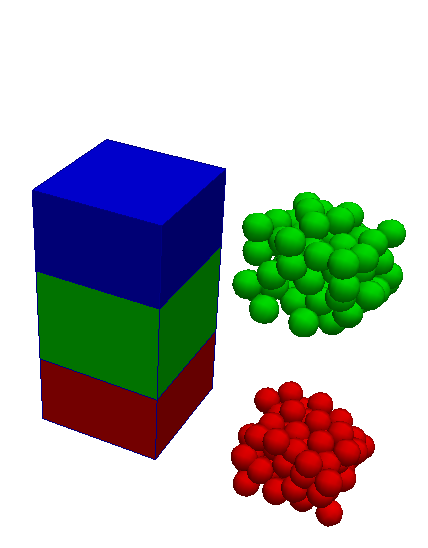
\includegraphics[height=7cm]{coupling/multi1/multi1-0050}}
\end{frame}


\subsection{Contact coupling}
\begin{frame}
	\frametitle{\secname}
	\framesubtitle{\subsecname}
	\centering
	\includegraphics[width=10cm]{raphaelpy/coupling_illustration_contact}
	\begin{picture}(0,0)
		\setlength{\unitlength}{10cm}
		\put(-0.8,.03){\makebox(0,0){DEM}}
		\put(-0.2,.03){\makebox(0,0){FEM}}
	\end{picture}
\end{frame}

\begin{frame}
	\frametitle{\secname}
	\framesubtitle{\subsecname}
	\centering
	\href{run:figs/contact1.gif}{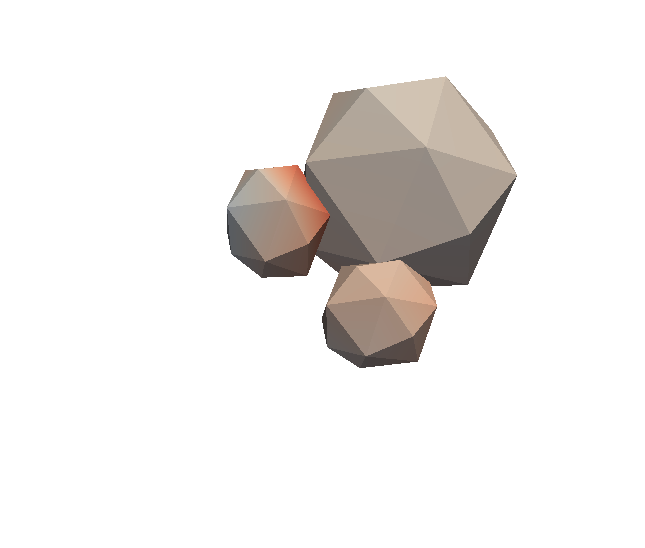
\includegraphics[height=7cm]{coupling/contact1/contact1-0053}}
\end{frame}
 
 
\subsection{Sequential coupling}
\begin{frame}
	\frametitle{\secname}
	\framesubtitle{\subsecname}
	\begin{twocolumns}
		\begin{onecolumn}
			\begin{myitemize}
				\item<1-> Processes separable in~time
				\item<4-> FEM model for concrete by Grassl \& Jirásek
				\item<5->
					DEM ($\stressTensor_{DEM},\damageTensor_{DEM}$)
					$\rightarrow$ 
					\par
					$\rightarrow$ 
					FEM ($\stressTensor,\damage,\kappaD,\kappaP$)
			\end{myitemize}
		\end{onecolumn}
		\begin{onecolumn}
			\only<1| handout:0>{\includegraphics[height=7cm]{figs/raphaelpy/sequential_coupling_illustration_0}}
			\only<2| handout:1>{
				\includegraphics[height=7cm]{figs/raphaelpy/sequential_coupling_illustration_1}
				\begin{picture}(0,0)
					\setlength{\unitlength}{1cm}
					\put(-.5,3.5){\makebox(0,0){DEM}}
				\end{picture}
			}
			\only<3| handout:2>{
				\includegraphics[height=7cm]{figs/raphaelpy/sequential_coupling_illustration_2}
				\begin{picture}(0,0)
					\setlength{\unitlength}{1cm}
					\put(-.5,3.5){\makebox(0,0){damage}}
					\put(-.8,5){\makebox(0,0){FEM}}
				\end{picture}
			}
			\only<4| handout:0>{
				\includegraphics[width=5cm]{../figs/raphaelpy/coupling_seq_cpm_dpm_2}
				\begin{picture}(0,0)
					\setlength{\unitlength}{5cm}
					\put(-0.1,0.05){\makebox(0,0)[r]{$\strain$}}
					\put(-0.88,0.566666666667){\makebox(0,0)[l]{$\stress$}}
					\put(-0.515,0.416666666667){\makebox(0,0)[l]{$\damage f_t$}}
					\put(-0.9,0.516666666667){\makebox(-.03,0)[r]{$f_t$}}
					\put(-0.95,-0.04){\makebox(0,0)[l]{$\damage=0$}}
					\put(-0.95,-0.10){\makebox(0,0)[l]{$\kappaD=0$}}
					\put(-0.95,-0.16){\makebox(0,0)[l]{$\kappaP<1$}}
					\put(-0.50,-0.04){\makebox(0,0)[l]{$\damage>0$}}
					\put(-0.50,-0.10){\makebox(0,0)[l]{$\kappaD>0$}}
					\put(-0.50,-0.16){\makebox(0,0)[l]{$\kappaP=\kappaD+1$}}
				\end{picture}
			}
			\only<5| handout:0>{
				\footnotesize
				$$
					\damageTensor = -\frac{1}{2}\trace{\damageTensor}\identityTensor2 + \frac{15}{2N}\sum_\contact\damageA^\contact\normalVector^\contact\otimes\normalVector^\contact =
				$$
				$$
					= -\identityTensor2\frac{3}{2N}\sum_\contact\damageA^\contact + \frac{15}{2N}\sum_\contact\damageA^\contact\normalVector^\contact\otimes\normalVector^\contact
				$$
				$$
					\damage_{FEM} = \damage(\damageTensor) = \damage(\damageTensorI_1,\damageTensorI_2,\damageTensorI_3)
				$$
				$$
					\kappaD = \kappaD(\damage),
					\kappaP = \kappaP(\damage)
				$$
			}
		\end{onecolumn}
	\end{twocolumns}
\end{frame}

\begin{frame}
	\frametitle{\secname}
	\framesubtitle{\subsecname}
	Results - uniaxial compression \par
	\centering
	\only<+| handout:0>{\inputplot{sequential_coupling_plain}}
	\only<+| handout:0>{
		\inputplot{sequential_coupling_001}
		\inputplot{sequential_coupling_002}
	}
	\only<+| handout:0>{
		\inputplot{sequential_coupling_004}
		\inputplot{sequential_coupling_005}
	}
	\only<+| handout:1>{
		\inputplot{sequential_coupling_007}
		\inputplot{sequential_coupling_009}
	}
\end{frame}


%%%%%%%%%%%%%%%%%%%%%%%%%%%%%%%%%%%%%%%%%%%%%%%%%%%%%%%%%%%%%%%%%%%%%%
% M C P M
%%%%%%%%%%%%%%%%%%%%%%%%%%%%%%%%%%%%%%%%%%%%%%%%%%%%%%%%%%%%%%%%%%%%%%
\section{Mesoscale DEM model for concrete}
\begin{frame}
	\frametitle{\secname}
	\begin{twocolumns}
		\begin{onecolumn}
			\begin{myitemize}
				\item three phase material
				\begin{myitemize}
					\item mortar matrix
					\item aggregate inclusions
					\item ITZ
				\end{myitemize}
				\item<2-> one material model
				\item<3-> 2 types of DEM particles
				\item<3-> 3 types of links
				\item<5-> ITZ link
				\begin{myitemize}
					\item weaker
					\item less stiff
					\item more brittle
				\end{myitemize}
			\end{myitemize}
		\end{onecolumn}
		\begin{onecolumn}
			\only<1| handout:0>{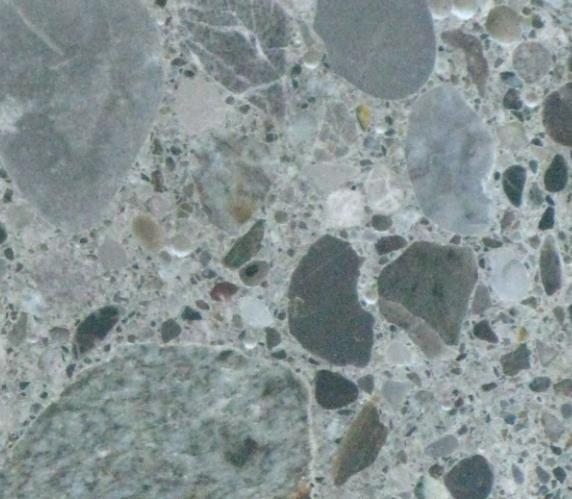
\includegraphics[width=\textwidth]{figs/concrete}}
			\only<2| handout:0>{
				\inputplot{cpm_law_tester_normal_simple_tension}
				\inputplot{cpm_shear_plasticity_func}
			}
			\only<3| handout:0>{\includegraphics[width=\textwidth]{../figs/raphaelpy/mcpm_itz_possibilities_1}}
			\only<4| handout:0>{\includegraphics[width=\textwidth]{../figs/raphaelpy/mcpm_itz_possibilities_0}}
			\only<5>{\includegraphics[width=\textwidth]{../figs/raphaelpy/mcpm_itz_possibilities_2}}
		\end{onecolumn}
	\end{twocolumns}
\end{frame}

\subsection{Validation}
\begin{frame}
	\frametitle{\secname}
	\framesubtitle{\subsecname}
	\begin{twocolumns}
		\begin{onecolumn}
			\begin{myitemize}
				\item<1-> Experiment Beygi et al.
				\item<1-> $\youngModulus$, $f_t$, $f_c$, $G_f$
				\item<2-> different grading curves
				\item<2-> same total amount of aggregates
				\item<3-> two types of concrete
			\end{myitemize}
		\end{onecolumn}
		\begin{onecolumn}
			\only<2>{
				\small
				\setlength\tabcolsep{.3em}
				\begin{tabular}{|c|c|c|c|}
					\hline
					max. aggreg & 9{.}5 & 12{.}5 & 19{.}0 \\
					\hline\hline
					powder          & 205 & 205 & 205 \\
					\hline
					sand            & 917 & 917 & 917 \\
					\hline
					4{.}75 - 9{.}5  & 750 & 300 & 300 \\
					\hline
					9{.}5 - 12{.}5  &  -  & 450 & 300 \\
					\hline
					12{.}5 - 19{.}0 &  -  &  -  & 150 \\
					\hline
				\end{tabular}
			}
			\only<3| handout:0>{
				\setlength\tabcolsep{.3em}
				\begin{tabular}{|c|c|c|}
					\hline
					 & $c$ & $w$ \\
					\hline\hline
					low s.  & 325{.}8 & 187{.}0 \\
					\hline
					high s. & 422{.}4 & 160{.}7 \\
					\hline
				\end{tabular}
			}
		\end{onecolumn}
	\end{twocolumns}
\end{frame}

\begin{frame}
	\frametitle{\secname}
	\framesubtitle{\subsecname}
	\only<1>{\inputplot{validationBeygi_l}}
	\only<2| handout:0>{\inputplot{validationBeygi_h}}
	\par
	\vspace{-5mm}
	\centering
	\inputplot{validationBeygi_legend}
	\vspace{-10mm}
\end{frame}


%%%%%%%%%%%%%%%%%%%%%%%%%%%%%%%%%%%%%%%%%%%%%%%%%%%%%%%%%%%%%%%%%%%%%%
% C O N C L U S I O N S
%%%%%%%%%%%%%%%%%%%%%%%%%%%%%%%%%%%%%%%%%%%%%%%%%%%%%%%%%%%%%%%%%%%%%%
\section{Conclusions}
\begin{frame}
	\frametitle{\secname}
	\only<1| handout:1>{
		\begin{block}{Conclusions}
			\begin{myitemize}
				\item macroscopic elastic properties of particle models
				\item discrete (couple) stress tensor
				\item DEM -- FEM coupling, new open source package
				\item sequential DEM -- FEM coupling
				\item mesoscale discrete element model for concrete
			\end{myitemize}
		\end{block}
	}
	\only<2| handout:2>{
		\begin{block}{Future work}
			\begin{myitemize}
				\item new formula for discrete couple stress tensor verification
				\item more detailed parameter study of MCPM
				\item more examples of sequential DEM -- FEM coupling
				\item more examples of concurrent DEM -- FEM coupling
			\end{myitemize}
		\end{block}
	}
\end{frame}


%%%%%%%%%%%%%%%%%%%%%%%%%%%%%%%%%%%%%%%%%%%%%%%%%%%%%%%%%%%%%%%%%%%%%%
% O P P O N E N T S
%%%%%%%%%%%%%%%%%%%%%%%%%%%%%%%%%%%%%%%%%%%%%%%%%%%%%%%%%%%%%%%%%%%%%%
\begin{discussion}
	
\section{Jan Eliáš}
\begin{questionframe}{1}
	\begin{questionblock}
		What other formulas for the evaluation of the couple stress tensor in a discrete system are used?
		What are their differences, advantages and disadvantages compared to the newly derived formula?
	\end{questionblock}
	\begin{answerblock}
		Bardet \& Vardoulakis and Chang \& Kuhn:
		\par
		\vspace{-3mm}
		$$
			\coupleStress_{ji}+\leviCivita{jkl}\Sigma_{jlk} = ...
		$$
		$$
			\Sigma_{kji}+\Sigma_{jki} = ...
		$$
		New formula
		\par
		\vspace{-3mm}
		$$
			\volume\volumeAverage{\coupleStressTensor}
			=
			\volume\centroidVector\otimes\br{\identityTensor2\cross\volumeAverage{\stressTensor}}
			+
			\sum_{\externalp}\positionVector\otimes\externalCoupleVector
		$$
	\end{answerblock}
\end{questionframe}

\begin{questionframe}{2}
	\begin{questionblock}
		Volume or surface coupling of discrete and continuum methods usually leads to undesirable reflection and dispersion of waves on their interface.
		Does any of the methods eliminate this problem?
	\end{questionblock}
	\begin{answerblock}
		No.
	\end{answerblock}
\end{questionframe}

\begin{questionframe}{3}
	\begin{questionblock}
		The mesoscale model presented in part 3 is composed of spherical particles.
		Their size has no physical interpretation and it seems that it may be chosen almost arbitrarily.
		Is the response of the model independent on the size of these particles?
	\end{questionblock}
	\begin{answerblock}
		\begin{myitemize}
			\item The model is NOT independent on particle size.
			\item For each particle size, the model should be calibrated independently.
		\end{myitemize}
	\end{answerblock}
\end{questionframe}

\begin{questionframe}{4}
	\only<1| handout:1>{
		\begin{questionblock}
			It is stated that it is possible to split the summation assuming uniform distribution of the product of contact areas and lengths in the equation 3.35.
			However, I have the impression that the distribution may be considered arbitrary.
			For the presented summation split, it is necessary to assume independence of the normal direction $\normalVector$ and the product of contact areas and lengths $\linkCrossSectionArea\linkLength$.
		\end{questionblock}
	}
	\only<2| handout:2>{
		\begin{answerblock}
			$$
				\stiffnessTensorElastic =
				\frac{1}{\volume} \sum_\contact \branch^\contact\linkCrossSectionArea^\contact\br{\linkMaterialStiffnessNormal\normalTensor4^\contact+\linkMaterialStiffnessShear\shearTensor4^\contact}
			$$
			$$
				\youngModulus =
				\frac{\sum\branch^\contact\linkCrossSectionArea^\contact}{3\volume}
				\cdot
				\frac{\linkMaterialStiffnessNormal\br{2\linkMaterialStiffnessNormal+3\linkMaterialStiffnessShear}}{4\linkMaterialStiffnessNormal+\linkMaterialStiffnessShear}
			$$
			$$
				\poissonRatio = \frac{\linkMaterialStiffnessNormal-\linkMaterialStiffnessShear}{4\linkMaterialStiffnessNormal+\linkMaterialStiffnessShear}
			$$	
			\begin{myitemize}
				\item I considered it as a part of the assumption of uniform distribution of link directions
				\item match of the results
				\item Least effect for low values of interaction ratio
			\end{myitemize}
		\end{answerblock}
	}
\end{questionframe}

\begin{questionframe}{5}
	\only<1| handout:1>{
		\begin{questionblock}
			Figures 3.8-3.11 show the difference of derived analytical formula and the real macroscopic response for low and high values of interaction ratio.
			Is there a simple explanation of the observed dependency on interaction ratio?
			Why is the estimation of elastic parameters so much different for low values of interaction ratio?
		\end{questionblock}
	}
	\only<2| handout:2>{
		\begin{answerblock}
			\inputplot{preprocessed_macromicro_E_I1.05}
			\inputplot{preprocessed_macromicro_nu_I1.05}
			\begin{myitemize}
				\item systematic error in my evaluation
				\item not fulfilled assumptions of the gray estimation
			\end{myitemize}
		\end{answerblock}
	}
	\only<3| handout:3>{
		\begin{questionblock}
			Is is possible to get such accurate estimation also for non-spherical particles (like ellipsoids) for the whole range of shear and normal stiffness?
		\end{questionblock}
		\begin{answerblock}
			I believe yes, but have not tested it nor did any research.
		\end{answerblock}
	}
\end{questionframe}


\section{Jan Zeman}
\begin{questionframe}{1}
	\begin{questionblock}
		Please, explain in more detail your statement from page 9:\par
		\textit{A~\quotes{small} change of positions of particles can cause a sudden (\quotes{big}) change of the stiffness of the system.
		For this reason, implicit integration schemes are in general not suitable for numerical solution and an explicit time integration scheme is usually applied to solve equations of motion}\par
	\end{questionblock}
	\begin{answerblock}
		\begin{myitemize}
			\item not very good expressions, \textit{not suitable} is too strong
			\item \textit{sudden change of stiffness} = zero or nonzero stiffness
			\item What I meant: explicit time integration is \quotes{less complex}
		\end{myitemize}
	\end{answerblock}
\end{questionframe}

\begin{questionframe}{2}
	\begin{questionblock}
		You assume an affine displacement of individual particles.
		This kinematic assumption is not fulfilled for heterogeneous materials because of perturbations of displacement field due to spatially variable stiffness.
		What is the influence of this assumption of the accuracy of obtained properties, with respect to the results presented in section 3.4.2?
	\end{questionblock}
	\begin{answerblock}
		\begin{myitemize}
			\item method is designed for homogeneous materials
			\item for heterogeneous material, each phase could be evaluated independently and another homogenization method could be used to determine overall elastic parameters.
		\end{myitemize}
	\end{answerblock}
\end{questionframe}

\begin{questionframe}{3}
	\begin{questionblock}
		Please, explain in more detail your statement on page 43:\par
		\textit{The resulting (couple) stress tensor does not depend on the choice of the point of moment equilibrium.}\par
		\textit{The resulting (couple) stress tensor does not depend on the choice of particles' reference points.}\par
	\end{questionblock}
	\begin{answerblock}
		These are necessary conditions for macro (couple) stress tensor according to Chang \& Kuhn.
	\end{answerblock}
\end{questionframe}

\begin{questionframe}{4}
	\begin{questionblock}
		Please, explain what you have tried to show with table 4.1 on page 46.
	\end{questionblock}
	\begin{answerblock}
		Simple illustration of (couple) stress tensor
		\centering
		\resizebox{.65\textwidth}{!}{%
			\def\w{2cm}
			\def\z{\cdot}
			\begin{tabular}{|C{2cm}|C{2cm}|C{2cm}|C{2cm}|C{2cm}|}
				\hline
				{} & $\stressTensor$ & $\coupleStressTensor$ \\
				\hline
				\hline
				%
				\includegraphics[width=\w]{raphaelpy/discrete_stress_0}
				&
				$\begin{bmatrix}
					\z & \z & \z \\
					\z & \z & \z \\
					\z & \z & \z \\
				\end{bmatrix}$
				&
				$\begin{bmatrix}
					\z & \z & \z \\
					\z & \z & \z \\
					\z & \z & \z \\
				\end{bmatrix}$
				\\
				\hline
				%
				\includegraphics[width=\w]{raphaelpy/discrete_stress_1}
				&
				$\begin{bmatrix}
					 2 & \z & \z \\
					\z & \z & \z \\
					\z & \z & \z \\
				\end{bmatrix}$
				&
				$\begin{bmatrix}
					\z & \z & \z \\
					\z & \z & \z \\
					\z & \z & \z \\
				\end{bmatrix}$
				\\
				\hline
				%
				\includegraphics[width=\w]{raphaelpy/discrete_stress_2}
				&
				$\begin{bmatrix}
					 1 & \z & \z \\
					\z & \z & \z \\
					\z & \z & \z \\
				\end{bmatrix}$
				&
				$\begin{bmatrix}
					\z & \z & \z \\
					\z & \z & \z \\
					\z & \z & \z \\
				\end{bmatrix}$
				\\
				\hline
				%
				\includegraphics[width=\w]{raphaelpy/discrete_stress_3}
				&
				$\begin{bmatrix}
					\z &  2 & \z \\
					 2 & \z & \z \\
					\z & \z & \z \\
				\end{bmatrix}$
				&
				$\begin{bmatrix}
					\z & \z & \z \\
					\z & \z & \z \\
					\z & \z & \z \\
				\end{bmatrix}$
				\\
				\hline
			\end{tabular}
			\hfill
			\begin{tabular}{|C{2cm}|C{2cm}|C{2cm}|C{2cm}|C{2cm}|}
				\hline
				{} & $\stressTensor$ & $\coupleStressTensor$ \\
				\hline
				\hline
				%
				\includegraphics[width=\w]{raphaelpy/discrete_stress_4}
				&
				$\begin{bmatrix}
					\z & \z & \z \\
					\z & \z & \z \\
					\z & \z & \z \\
				\end{bmatrix}$
				&
				$\begin{bmatrix}
					\z & \z &  2 \\
					\z & \z & \z \\
					\z & \z & \z \\
				\end{bmatrix}$
				\\
				\hline
				%
				\includegraphics[width=\w]{raphaelpy/discrete_stress_5}
				&
				$\begin{bmatrix}
					\z & \z & \z \\
					\z & \z & \z \\
					\z & \z & \z \\
				\end{bmatrix}$
				&
				$\begin{bmatrix}
					\z & \z &  1 \\
					\z & \z & \z \\
					\z & \z & \z \\
				\end{bmatrix}$
				\\
				\hline
				%
				\includegraphics[width=\w]{raphaelpy/discrete_stress_6}
				&
				$\begin{bmatrix}
					\z &  2 & \z \\
					\z & \z & \z \\
					\z & \z & \z \\
				\end{bmatrix}$
				&
				$\begin{bmatrix}
					\z & \z & \z \\
					\z & \z & \z \\
					\z & \z & \z \\
				\end{bmatrix}$
				\\
				\hline
				%
				\includegraphics[width=\w]{raphaelpy/discrete_stress_7}
				&
				$\begin{bmatrix}
					\z & \z & \z \\
					 1 & \z & \z \\
					\z & \z & \z \\
				\end{bmatrix}$
				&
				$\begin{bmatrix}
					\z & \z & \z \\
					\z & \z & \z \\
					\z & \z & \z \\
				\end{bmatrix}$
				\\
				\hline
			\end{tabular}
			}
	\end{answerblock}
\end{questionframe}

\begin{questionframe}{5}
	\only<1| handout:1>{
		\begin{questionblock}
			Please, explain based on which considerations you got the calibration formulas in equations (6.17)-(6.19)
		\end{questionblock}
	}
	\only<2| handout:2>{
		\begin{answerblock}
			$$
				\damage = 2{.}09\br{0{.}85\damageTensorI_1+0{.}15\damageTensorI_3}^{4{.}7}
			$$
			\centering
			\inputplot{sequential_coupling_dmg}
		\end{answerblock}
	}
	\only<3| handout:3>{
		\begin{answerblock}
			\vspace{-5mm}
			$$
				\text{if}\quad \damage \le m \quad \text{then}\quad \kappaD = 0, \kappaP = \kappaP(\damage), \damage = 0
			$$
			$$
				m = 5\cdot10^{-4},\quad \kappaP = 0{.}3 + 900\damage
			$$
			\centering
			\par
			\vspace{-3mm}
			\inputplot{sequential_coupling_002}
		\end{answerblock}
	}
\end{questionframe}

\begin{questionframe}{6}
	\begin{questionblock}
		Results in figure 8.6 should be explained better.
		For example, it is not clear what is the meaning of the vertical axis and how the results reflects the influence of the transition zone (as was declared in the objectives of the doctoral thesis).
	\end{questionblock}
	\begin{answerblock}
		\begin{myitemize}
			\item \textit{Since the absolute values of macroscopic quantities can be relatively easily estimated, only values relative to the results for the smallest aggregate size are plotted.}
			\item More detailed parameter study could be done to assess influence of ITZ.
		\end{myitemize}
	\end{answerblock}
\end{questionframe}

\end{discussion}

\end{document}
